\documentclass[12pt]{article}
\usepackage[utf8]{inputenc}
\usepackage{amsmath, amssymb, physics, graphicx, tikz}
\usepackage[a4paper, margin=1in]{geometry}
\usepackage{fancyhdr}
\usepackage{hyperref}
\usepackage{xcolor}
\definecolor{sectionrectanglecolor}{rgb}{0.25,0.5,0.75}
\definecolor{sectiontitlecolor}{rgb}{0.2,0.4,0.65}
\definecolor{subsectioncolor}{rgb}{0,0,0}
\definecolor{lightgray}{gray}{0.9}
\definecolor{darkgray}{gray}{0.1}
\definecolor{lightred}{rgb}{0.9,0,0.1}
\usepackage{wrapfig}
\usepackage{tcolorbox}
\graphicspath{{Figures/}{../Figures/}}

\newcommand{\be}{\begin{eqnarray}}
\newcommand{\non}{\nonumber \\ }
\newcommand{\ee}{\end{eqnarray}}
\newif\ifshowboardanswers
\showboardanswersfalse
% Set this to \showboardquestiontrue to include the end-of-lecture board question.
\newif\ifshowboardquestion
\showboardquestionfalse
\newcommand{\boardanswer}[1]{\ifshowboardanswers\\[0.35em]\textcolor{blue}{\textbf{Answer.} #1}\fi}

\fancyhead[L]{Special Relativity}
\fancyhead[R]{Lecture 3}
\setlength{\headheight}{14.5pt}

\title{\textbf{Lecture 3: Lorentz Transformations}}
\author{Based on Morin's \textit{Introduction to Classical Mechanics}, Ch. 11.4--11.5}
\date{}

\begin{document}
\maketitle

\section*{Outline}
\begin{enumerate}
    \item \href{sec:recap}{Recap lecture 2}
    \item \href{sec:diagramtoolkit}{Diagram toolkit for transformations}
    \item \href{sec:LT}{Lorentz Transformations}
    \item \href{sec:EVT}{Einstein Velocity Transformations}
\end{enumerate}

\section{Recap Lecture 2}\label{sec:recap}
\subsection{Events}
An \textbf{event} is a specific point in spacetime, defined by:
\[
(t, x, y, z).
\]
It occurs at a particular location and instant in time (which we have to add to our `position' vector). Events are the basic entities in relativity. All observers agree on whether two events occurred at the same place and time in their own frame, but may disagree on the simultaneity of events between frames. This is the reason why time has to be added. Since this time is frame dependent (as we saw in lecture 2), we refer to this time as {\bf coordinate time}. Since $\gamma \geq 1$, the clock for an observer at rest runs faster ($t \geq t'$). They are equal only if two observers are at rest with respect to each other (i.e., $S = S'$).

\subsection{Time Dilation}
Derived from the light clock in lecture 2:
\begin{equation}
t= \gamma t', \quad \text{where } \gamma = \frac{1}{\sqrt{1 - v^2/c^2}}
\end{equation}
% \textbf{Proper time} $t_0$ is the time interval measured in the frame where the clock is at rest.
Note that the above is assuming there is some zero point time, since this relation really only applies to intervals, i.e. $\Delta t \equiv t_2 - t_1$, where $t_2 > t_1$. Hence, the above implicitly assumes $t_1 =0$.  I am writing it like this here, since Morin tends to drop the $\Delta$. 




\subsection{Muon Decay}
Muons created in the upper atmosphere have a half-life time $t_{1/2}' = 1.5\,\mu s$ in their rest frame $S'$. They travel at $v = 0.99c$. These cosmic muons are created at a height of $60$ km in the atmosphere. In a Galilean Universe, we would argue that it would take 
\be
\Delta t = \Delta h / v = 60\;{\rm km}/ (0.99 c) \sim 200 \mu{\rm s}
\ee
to reach Earth. Given the half-life, you would thus get that 
\be
N \times \left(\frac{1}{2}\right)^{200/1.5} = 1 \rightarrow N = 2^{200/1.5} \sim 10^{40}. 
\ee
So 1 in $10^{40}$ muons is expected to reach Earth. 

In SR, the lifetime is measured in the frame that is at rest with respect to the Muon $S'$. So we need to fold in time dilation (or length contraction, both work). 

In the Earth's frame $S$, the lifetime of the muon is actually longer by
\be
\gamma(v = 0.99c) \simeq 7 \rightarrow t_{1/2} \simeq 10.5\;\mu{\rm s}.
\ee
If SR is correct, we thus conclude that 
\be
N \sim 2^{200/10.5} \sim 5\times 10^5.  
\ee
So over 1 in $500.000$ reaches Earth, which matches observations. 
% \section{Proper Time}


\subsection{Length Contraction}
\textbf{Proper length} $L_0$: Length measured in the frame where the object is at rest.

We derived that the length of an object that is moving with respect to an observer at rest is contracted: 
\begin{equation}
L = L_0 \sqrt{1 - v^2/c^2} = \frac{L_0}{\gamma}.
\end{equation}
Since $\gamma \geq 1$, $0\leq \gamma^{-1}\leq 1$, i.e., the length is contracted. Only for a (hypothetical) object that would move at $c$, the length would be contracted to zero. 

\subsection*{Example 2: High-Speed Train}
A train of proper length $L_0 = 500$ m moves at $v = 0.8c$. Find its length in the ground frame.

\begin{align*}
\gamma &= \frac{1}{\sqrt{1 - 0.64}} = \frac{1}{0.6} \approx 1.667 \\
L &= \frac{500}{1.667} \approx 300 \text{ m}
\end{align*}
Note that while the train is already moving close to the speed of light, length contraction is still relatively minor. Since the Lorentz factor scales as the square root of the velocity, the velocity has to get exponentially close to $c$ to get large effects. It is also the reason why, in everyday life, we have no experience with relativistic effects. 

\section{Diagram toolkit for transformations}\label{sec:diagramtoolkit}
Before deriving the Lorentz transformations algebraically, it is useful to know what the answer should look like on a spacetime diagram. Figure~\ref{fig:two-observer-diagram} shows the two-observer diagram that we will use as a guide. We use units with $c=1$, so light rays always have slope $\pm 1$.

\begin{figure}
\begin{center}
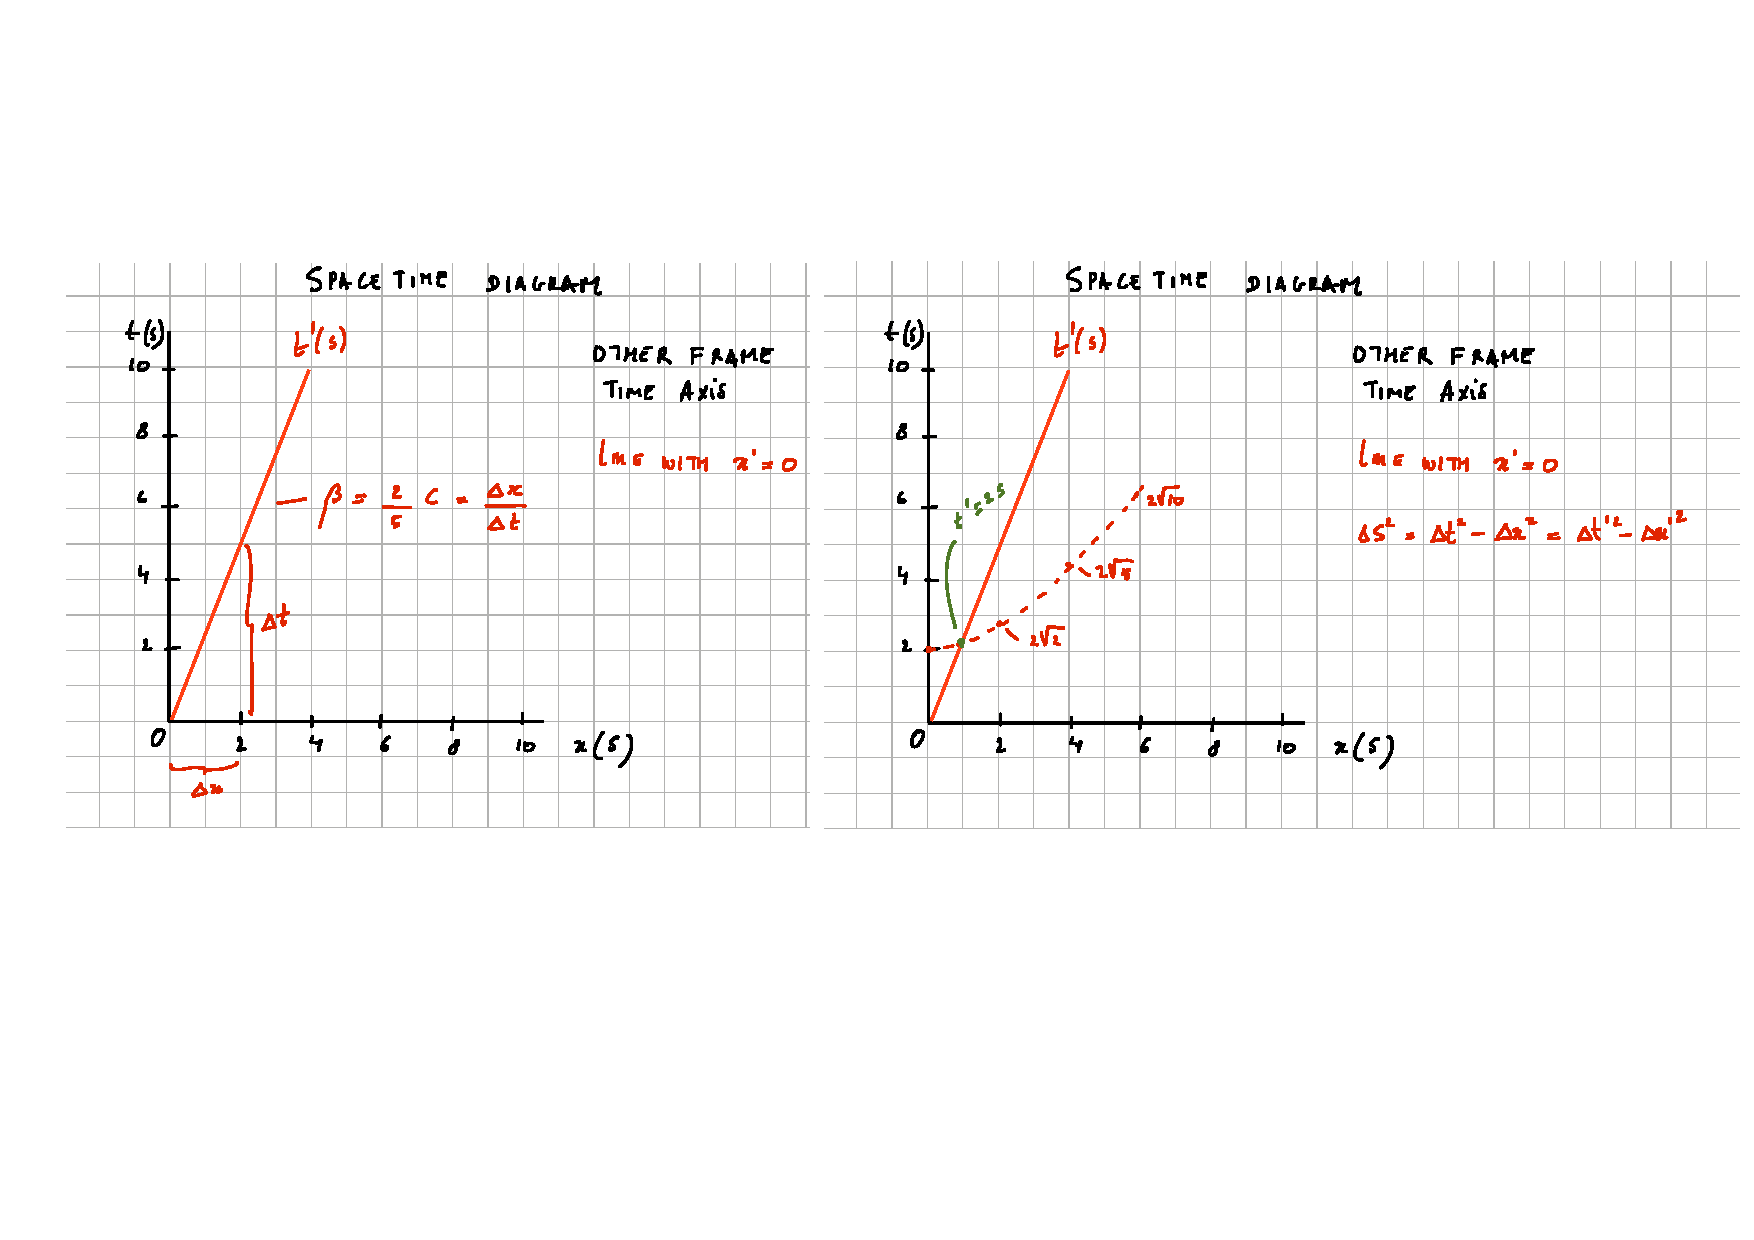
\includegraphics[width=0.88\textwidth]{2ODa.pdf}
\end{center}
\caption{A two-observer diagram. The unprimed frame $S$ uses the vertical $t$ axis and horizontal $x$ axis. The moving frame $S'$ uses tilted $t'$ and $x'$ axes.}
\label{fig:two-observer-diagram}
\end{figure}

\begin{itemize}
    \item The $t'$ axis is the worldline of the origin of $S'$. If $S'$ moves with velocity $v$ in $S$, then this line satisfies $x=vt$.
    \item The $x'$ axis is the set of events that are simultaneous with $t'=0$ in the moving frame. It tilts by the same amount toward the light cone as the $t'$ axis.
    \item The light cone is not tilted by a change of inertial frame. This is the geometric statement that all inertial observers measure the same speed of light.
    \item Lines of constant $x'$ are parallel to the $t'$ axis; lines of constant $t'$ are parallel to the $x'$ axis.
\end{itemize}

The important lesson is that a Lorentz transformation is not a rotation in the Euclidean sense. It tilts the time and space axes toward the light cone while preserving the spacetime interval. This picture should be kept next to the algebra below: the equations tell us how to compute coordinates, while the diagram tells us what the computation means.

\section{Lorentz transformations}\label{sec:LT}
In Moore, the Lorentz transformations are derived only in {\bf Chapter 5}. In Morin, they are derived in {\bf section 5} of the first chapter. We will first use the spacetime diagram above as a guide, and then follow Morin's algebraic derivation. We will use some of the things we have just learned about clocks and lengths. 

A key point in SR is that, unlike Galilean Relativity, space and time are interwoven. We know a priori that we move both through space and time. While time is absolute and unchanging for observers in different inertial frames, this will not hold in SR. From Galilean transformation rules, we know that a transformation is simply some (mathematical) relation between the coordinates in one frame $S$ and another frame $S'$. Suppose that $S'$ is moving to the right (positive velocity), which we will call $v$. We will use (un-) primed coordinates $(t',x')$ ($(t,x)$) for frame $S'$ ($S$). We will ignore the two other spatial directions, as we have learned that space (length) is not affected in those directions if there is no motion in that direction. Given the example of Galilean transformations, we are going to make an ansatz about the transformation rules in SR, which are: 
\be
\Delta x  &=& A \Delta x' + B \Delta t',\\
\Delta t  &=& C \Delta t' + D \Delta x'. 
\ee
Our goal will be to determine the constants $A,B,C$, and $D$. Like Galilean transformations, these functions will depend on $v_x \equiv v$, the velocity of frame $S'$ as measured in frame $S$.

To determine these constants, we can take limiting cases in which we know the answer. First, consider no displacement in frame $S'$, i.e., $\Delta x' = 0$. In this case, we can use our knowledge of time dilation:
\be
\Delta t  = \gamma\Delta t'. 
\ee
In other words, $C = \gamma$ (that was easy!). 

Next, let us consider length contraction. In that case, we should set $\Delta t' = 0$, while 
\be
\Delta x' = \gamma^{-1} \Delta x.
\ee
Hence $A = \gamma$. 

Now things will get a little bit trickier. Suppose I am an observer in frame $S$ and I am not moving ($\Delta x = 0$). What is my velocity in the other frame? That is easy, it should be $-v$ (since I am at rest and the other frame $S'$ has velocity $v$). The velocity in that other frame should be determined via $\Delta x'/\Delta t' = -v$. This implies that $B/A = v$ or $B = \gamma v$. 

Finally, we need to derive a relation that is valid when $\Delta t = 0$, meaning that two events are simultaneous in observer A's rest frame $S$. Morin refers to the resulting effect as rear-clock ahead: when the rear and front arrival events are simultaneous in $S$, the clock at the rear of the moving train reads later than the clock at its front. The train is at rest in $S'$, not in A's frame $S$. I alluded to this example in Lecture 2. It goes as follows.

\begin{figure}
\begin{center}
\tikzset{every picture/.style={line width=0.75pt}} %set default line width to 0.75pt        

    
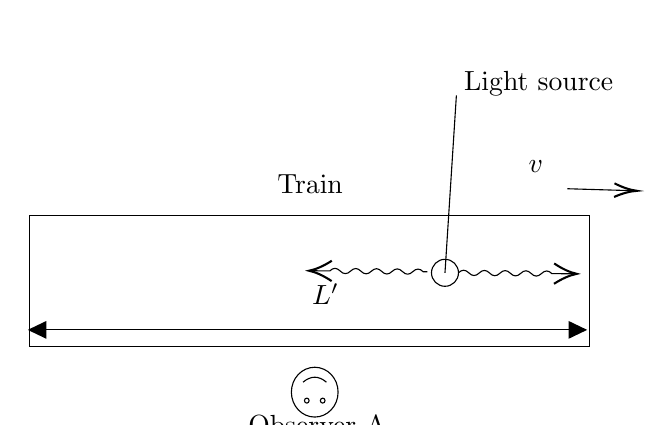
\begin{tikzpicture}[x=0.75pt,y=0.75pt,yscale=-1,xscale=1]
%uncomment if require: \path (0,300); %set diagram left start at 0, and has height of 300

%Shape: Rectangle [id:dp6337164416546507] 
\draw   (155,103) -- (424.5,103) -- (424.5,166) -- (155,166) -- cycle ;
%Straight Lines [id:da9430988568200938] 
\draw    (414,90) -- (445.5,90.94) ;
\draw [shift={(447.5,91)}, rotate = 181.71] [color={rgb, 255:red, 0; green, 0; blue, 0 }  ][line width=0.75]    (10.93,-3.29) .. controls (6.95,-1.4) and (3.31,-0.3) .. (0,0) .. controls (3.31,0.3) and (6.95,1.4) .. (10.93,3.29)   ;
%Shape: Circle [id:dp09048670053759289] 
\draw   (348.5,130.5) .. controls (348.5,126.91) and (351.41,124) .. (355,124) .. controls (358.59,124) and (361.5,126.91) .. (361.5,130.5) .. controls (361.5,134.09) and (358.59,137) .. (355,137) .. controls (351.41,137) and (348.5,134.09) .. (348.5,130.5) -- cycle ;
%Straight Lines [id:da7296346919962876] 
\draw    (157,158) -- (420.5,158) ;
\draw [shift={(423.5,158)}, rotate = 180] [fill={rgb, 255:red, 0; green, 0; blue, 0 }  ][line width=0.08]  [draw opacity=0] (8.93,-4.29) -- (0,0) -- (8.93,4.29) -- cycle    ;
\draw [shift={(154,158)}, rotate = 0] [fill={rgb, 255:red, 0; green, 0; blue, 0 }  ][line width=0.08]  [draw opacity=0] (8.93,-4.29) -- (0,0) -- (8.93,4.29) -- cycle    ;
%Straight Lines [id:da10692885328779789] 
\draw    (361.5,130.5) .. controls (363.18,128.85) and (364.85,128.86) .. (366.5,130.54) .. controls (368.15,132.22) and (369.82,132.24) .. (371.5,130.59) .. controls (373.18,128.94) and (374.85,128.95) .. (376.5,130.63) .. controls (378.15,132.31) and (379.82,132.33) .. (381.5,130.68) .. controls (383.18,129.03) and (384.85,129.04) .. (386.5,130.72) .. controls (388.15,132.4) and (389.82,132.41) .. (391.5,130.76) .. controls (393.18,129.11) and (394.85,129.13) .. (396.5,130.81) .. controls (398.15,132.49) and (399.82,132.5) .. (401.5,130.85) .. controls (403.18,129.2) and (404.85,129.21) .. (406.5,130.89) -- (408.5,130.91) -- (416.5,130.98) ;
\draw [shift={(418.5,131)}, rotate = 180.5] [color={rgb, 255:red, 0; green, 0; blue, 0 }  ][line width=0.75]    (10.93,-4.9) .. controls (6.95,-2.3) and (3.31,-0.67) .. (0,0) .. controls (3.31,0.67) and (6.95,2.3) .. (10.93,4.9)   ;
%Straight Lines [id:da3272651345513109] 
\draw    (291.5,129.52) -- (299.5,129.59) .. controls (301.18,127.94) and (302.85,127.95) .. (304.5,129.63) .. controls (306.15,131.31) and (307.82,131.33) .. (309.5,129.68) .. controls (311.18,128.03) and (312.85,128.04) .. (314.5,129.72) .. controls (316.15,131.4) and (317.82,131.41) .. (319.5,129.76) .. controls (321.18,128.11) and (322.85,128.13) .. (324.5,129.81) .. controls (326.15,131.49) and (327.82,131.5) .. (329.5,129.85) .. controls (331.18,128.2) and (332.85,128.21) .. (334.5,129.89) .. controls (336.15,131.57) and (337.82,131.59) .. (339.5,129.94) .. controls (341.18,128.29) and (342.85,128.3) .. (344.5,129.98) -- (346.5,130) -- (346.5,130) ;
\draw [shift={(289.5,129.5)}, rotate = 0.5] [color={rgb, 255:red, 0; green, 0; blue, 0 }  ][line width=0.75]    (10.93,-4.9) .. controls (6.95,-2.3) and (3.31,-0.67) .. (0,0) .. controls (3.31,0.67) and (6.95,2.3) .. (10.93,4.9)   ;
%Straight Lines [id:da24023633678733602] 
\draw    (355,130.5) -- (360.5,45) ;
%Shape: Smiley Face [id:dp35037367928330254] 
\draw   (303.5,188) .. controls (303.5,194.63) and (298.46,200) .. (292.25,200) .. controls (286.04,200) and (281,194.63) .. (281,188) .. controls (281,181.37) and (286.04,176) .. (292.25,176) .. controls (298.46,176) and (303.5,181.37) .. (303.5,188) -- cycle ; \draw   (297.2,192.08) .. controls (297.2,192.74) and (296.7,193.28) .. (296.08,193.28) .. controls (295.45,193.28) and (294.95,192.74) .. (294.95,192.08) .. controls (294.95,191.42) and (295.45,190.88) .. (296.08,190.88) .. controls (296.7,190.88) and (297.2,191.42) .. (297.2,192.08) -- cycle ; \draw   (289.55,192.08) .. controls (289.55,192.74) and (289.05,193.28) .. (288.43,193.28) .. controls (287.8,193.28) and (287.3,192.74) .. (287.3,192.08) .. controls (287.3,191.42) and (287.8,190.88) .. (288.43,190.88) .. controls (289.05,190.88) and (289.55,191.42) .. (289.55,192.08) -- cycle ; \draw   (297.88,183.2) .. controls (294.12,180) and (290.37,180) .. (286.63,183.2) ;

% Text Node
\draw (394,75) node [anchor=north west][inner sep=0.75pt]    {$v $};
% Text Node
\draw (273,82) node [anchor=north west][inner sep=0.75pt]   [align=left] {Train};
% Text Node
\draw (289.75,134.5) node [anchor=north west][inner sep=0.75pt]    {$L'$};
% Text Node
\draw (363,32) node [anchor=north west][inner sep=0.75pt]   [align=left] {Light source};
% Text Node
\draw (259,198) node [anchor=north west][inner sep=0.75pt]   [align=left] {Observer A};


\end{tikzpicture}
\caption{A train of length $L'$ (as measured at rest in frame $S'$) is moving to the right with velocity $v$. A source on the train is emitting two pulses. They arrive at the rear and front of the train at the same time, as observed (by observer `A') in the rest frame $S$. Figure taken from R2, 2023-2024. }
\label{fig:rca}
\end{center}
\end{figure}

Consider the setup as shown in Fig.~\ref{fig:rca}, where a train is moving with velocity $v$. The train has length $L'$ (as measured at rest -- proper length). 
Two light rays/pulses are submitted to the rear and front of the train, which arrive simultaneously for observer A ($\Delta t = 0$). Light rays appear to move $c+v$ to the back of the train and $c-v$ to the front of the train. This is ok, since it is really the distance between the location of the emitted pulse and the front and rear of the train that is changing; the rear is moving towards this point with velocity $v$, while the front is moving away from this point with velocity $v$. 

Now that we have convinced ourselves that this makes sense (Morin comments on this also), we can also write a relative relation between the distances to the front and rear of the train from the emitter:
\be
\frac{D'_{\rm back}}{D'_{\rm front}} = \frac{c+v}{c-v} = \frac{1+\beta}{1-\beta}, 
\ee
where I have divided by $c$ and defined $\beta = v/c$ for now.
At the same time, we know:
\be
D'_{\rm back} + D'_{\rm front} = L'.
\ee
Hence 
\be
D'_{\rm back} = \frac{1+\beta}{1-\beta} D'_{\rm front},
\ee
and 
\be
 D'_{\rm back} + D'_{\rm front}  = (\frac{1+\beta}{1-\beta}+1) D'_{\rm front}  = (\frac{1+\beta}{1-\beta} + \frac{1-\beta}{1-\beta})D'_{\rm front}  = \frac{2}{1-\beta} D'_{\rm front}.
\ee
This tells us that $D'_{\rm front} = L'(1-\beta)/2$ and 
\be
D'_{\rm back} = L' - D'_{\rm front} = L' - \frac{L'(1-\beta)}{2} = L'(1-\frac{1-\beta}{2}) = \frac{L'(1+\beta)}{2}.
\ee
Then we compute the ‘extra’ distance the light has to move to the back of the train:
\be
 D'_{\rm back} - D'_{\rm front} = L' \frac{1+\beta}{2} - L' \frac{1-\beta}{2} = \beta L'.
\ee
Putting $c$ back in and realizing (rear-clock-ahead):
\be
\Delta t' = t_{\rm front}-t_{\rm back} = -(D'_{\rm back} - D'_{\rm front})/c,
\ee
we find:
\be
\Delta t'  = -v \Delta x' /c^2. 
\ee
This allows us to find that $D/C = v/c^2$ and hence $D = \gamma v/c^2$. 
The Lorentz transformations are thus given by:
\begin{tcolorbox}[colback=blue!5!white]
\vspace{-1.3em}
\begin{align}
\Delta x &= \gamma (\Delta x' + v \Delta t')\label{eq:xLT} \\
\Delta t &= \gamma (\Delta t' +  v\Delta x' /c^2) \label{eq:tLT},
\end{align}
and (for completeness)
\be
\Delta y &=& \Delta y' \\
\Delta z &=& \Delta z'.
\ee
\end{tcolorbox}
\noindent 
These transformation rules are the cornerstone of SR, and from these, everything about SR can be derived (including, e.g., the velocity transformation as we will see soon). In SR units, $c = 1$ and the transformations become completely symmetric, showing indeed that space and time are treated identically in SR. Both spatial and temporal intervals are frame dependent, but we can relate them using the above equations. We will later discuss that in fact we can define something that is frame independent (namely the (spacetime) interval -- also proper time), but such a quantity necessarily will have to depend on both spatial and temporal intervals. The existence of such an invariant interval (and its definition) allows us to derive the Lorentz transformation in a different way (something we might discuss at some point, see e.g., Lecture 8 from 2024 year and R2 from 2023-2024). 

We can consider the limit $v\rightarrow 0$. In that case, we know $\gamma \rightarrow 1$ and $\Delta t = \Delta t'$ (as $v/c^2 \ll 1$) while $\Delta x = \Delta x' + v \Delta t'$, i.e., the Galilean transformations. 

\subsection{Matrix notation}
We can write the Lorentz transformation in matrix notation if we use SR units:
\be
\begin{pmatrix}
\Delta x' \\
\Delta t'
\end{pmatrix} =
\begin{pmatrix}
\gamma & -\beta \gamma \\
-\beta \gamma  & \gamma
\end{pmatrix}\begin{pmatrix}
\Delta x \\
\Delta t
\end{pmatrix},
\ee
with $\beta = v/c$.  Note that I have considered the inverse transformations (going from frame $S$ to $S'$). In that case we pick up a minus sign in the velocity, since from the perspective of an observer at rest in frame $S'$, anyone comoving\footnote{I will often use comoving, which often is short-hand for stating that an observer is at rest with respect to some coordinate frame, and moving with (=comoving) the frame as observed from any other inertial reference frame.} with frame $S$ is now moving in the opposite direction.  
This looks very similar to a rotation matrix. Coordinates in a (Cartesian) plane $x,y$ can be related to coordinates in a plane that is rotated around its origin with an angle $\alpha$ 
\begin{align*}
x_A' &= x_A \cos \alpha + y_A \sin \alpha, \\
y_A' &= -x_A \sin \alpha + y_A \cos \alpha.
\end{align*}
This can be written as 
\be
\begin{pmatrix}
x' \\
y'
\end{pmatrix} =
\begin{pmatrix}
\cos \alpha &  \sin \alpha \\
-\sin \alpha & \cos \alpha
\end{pmatrix}
\begin{pmatrix}
x \\
y
\end{pmatrix}.
\ee
We will discuss this analogy later when we talk about rapidity in lecture 5. This can be particularly useful if you want to show that applying $n$ (with $n>1$) Lorentz transformations can still be expressed as a Lorentz transformation, albeit with the appropriately transformed velocity. There are multiple old exam questions on this topic, which involve pretty tedious algebra (see e.g. R3, 2023-2024, Question 1). With rapidity, such problems become trivial. 

\subsection{Fundamental effects revisited}

\subsubsection{Loss of simultaneity}
If two events (at e.g., coordinates $(t_1',x_1')$, $(t_2',x_2'))$ occur simultaneously in frame $S'$, we know $(\Delta t',\Delta x') = (0,\Delta x')$, i.e. $t_1'=t_2'$. Using Eq.~\eqref{eq:tLT}, we find that in $S$, $\Delta t= \gamma v \Delta x'/c^2$. Unless $\Delta x' = 0$, the events therefore do not happen simultaneously in frame $S$.

\subsubsection{Time Dilation}
Now consider two ticks of a clock at rest in frame $S'$. These events have $(\Delta t', \Delta x'=0)$. In frame $S$, Eq.~\eqref{eq:tLT} gives $\Delta t = \gamma \Delta t'$. This is time dilation: according to an observer in frame $S$, a clock in frame $S'$ runs slow.

\noindent 
The reciprocal statement is also true: if we consider two ticks of a clock at rest in $S$, then $\Delta x=0$. Using the inverse Lorentz transformation gives $\Delta t' = \gamma \Delta t$. Thus an observer in $S'$ judges the clock at rest in $S$ to run slow. This is not a contradiction: the two statements concern different pairs of events---events at one location in $S'$ in the first case, and events at one location in $S$ in the second.

To compare the total elapsed times on two clocks directly, the clocks must later meet again. If two observers separate with constant relative velocity, at least one must change velocity for a reunion to occur. In the standard twin-paradox setup, this change of motion breaks the symmetry. The clock readings at reunion are determined by the total time recorded by each clock along its journey; the travelling clock records less elapsed time.

\subsubsection{Length Contraction}

Recall that an object's length in a given inertial frame is defined to be the distance between any two simultaneous events that occur at its ends. Hence, we need to be concerned with measurements of $\Delta t'$ that are zero in one frame. Let us consider an object of length $L'$ in frame $S'$. To find the length of that object in frame $S$, we set $\Delta t=0$ and use inverse of Eq.~\eqref{eq:xLT} to find $\Delta x' = \gamma \Delta x$ which implies $L = \gamma^{-1} L'$, the length of an object of length $L'$ in frame $S'$ is contracted in frame $S$. The reverse is also true (length $L$ in frame $S$ appears constructed in frame $S'$, something that can be shown using a {\bf two observer} diagram very easily. We will come back to this once we introduce diagrams. 

\section{Einstein velocity transformations}\label{sec:EVT}
We have shown how coordinates transform in the previous section. Here, we aim to show how velocities transform. Take two frames $S$ and $S'$, and $S'$ is moving with velocity $u$ (in the positive $x$ direction). An object in frame $S'$ is moving with velocity $v'$ in that frame. What is the velocity of that object as observed in $S$? We can simply use the LT we just derived. In $S$ the velocity can be written as $v \equiv \frac{dx}{dt} = \frac{\Delta x}{\Delta t}$:
\be
v = \frac{\Delta x}{\Delta t} = \frac{\gamma (\Delta x' + u \Delta t')}{\gamma (\Delta t' +  u\Delta x' /c^2)} = \frac{\frac{\Delta x'}{\Delta t'}+u}{1+u \frac{\Delta x'}{\Delta t'}/c^2} \equiv \frac{v' + u}{1+u v'/c^2},
\ee
where I used that $\Delta x'/\Delta t' = v'$. This is the longitudinal velocity addition rule (since the motion of the object is parallel to the motion of the frame $S'$). Note that if either $v' = c$ or if $u  = c$, $v = c$. This should be the case! One of the postulates of SR is that nothing can move faster than the speed of light, even something that is already moving with the speed of light in a frame that is at non-zero speed. We could also interchange $v'$ and $u$, it does not matter whether you interchange the motion of the frame and the object within that frame. If both $u$ and $v'$ are less than $c$, $v < c$. In the case we take small velocities compared to $c$, the denominator $1+ uv'/c^2\rightarrow 1$ and $v \simeq v'+u$, i.e., the classical result.

\subsection*{Worked example: two overtaking trains}
Two trains, $a$ and $b$, each have rest length $L$. In a reference frame $S$, both move to the right with speeds $v_a>v_b$, so train $a$ overtakes train $b$. The example illustrates a useful habit: first choose the frame in which the geometry of the question is simplest.

\paragraph{Part 1: How long does the overtaking take?}
Choose the frame $S_b$ comoving with train $b$. Train $b$ is then at rest, and train $a$ approaches with the relative speed
\be
w \equiv v_{a,b} = \frac{v_a-v_b}{1-v_a v_b/c^2}.
\ee
In $S_b$, train $a$ is length-contracted while train $b$ retains its rest length. Thus
\be
L_a^{(b)} = \frac{L}{\gamma_w}=L\sqrt{1-w^2/c^2},
\ee
where $\gamma_w=(1-w^2/c^2)^{-1/2}$. For train $a$ to pass train $b$ completely, it must travel the distance
\be
D=L+L_a^{(b)}.
\ee
Therefore the elapsed time in the frame of train $b$ is
\be
\Delta t_b = \frac{D}{w}=\frac{L(1+\gamma_w^{-1})}{w}.
\ee
For $v_a=4c/5$ and $v_b=3c/5$, we find $w=5c/13$, $\gamma_w=13/12$, and hence
\be
\Delta t_b=\frac{5L}{c}.
\ee

\paragraph{Part 2: What time does a walking observer measure?}
An observer $O$ walks from the rear to the front of train $b$. They begin walking at event $E_1$, when the front of train $a$ reaches the rear of train $b$, and arrive at the front of train $b$ at event $E_2$, when the rear of train $a$ passes it. We want the elapsed time between $E_1$ and $E_2$ in the rest frame of $O$.

In this frame the two trains have equal speeds in opposite directions; call the magnitude of either speed $v_O$. Their relative speed must still equal $w$, so the velocity-addition formula gives
\be
\frac{2v_O}{1+v_O^2/c^2}=w=\frac{v_a-v_b}{1-v_a v_b/c^2}.
\ee
Solving this equation and selecting the physical root, $|v_O|<c$, gives
\be
v_O=\frac{c^2-v_av_b-\sqrt{c^4-c^2(v_a^2+v_b^2)+v_a^2v_b^2}}{v_a-v_b}.
\ee
For $v_a=4c/5$ and $v_b=3c/5$, this yields $v_O=c/5$ and $\gamma_O=5/(2\sqrt{6})$. In $O$'s frame, train $b$ has length $L/\gamma_O$. Since $O$ crosses this contracted length at speed $v_O$,
\be
\Delta t_O=\frac{L/\gamma_O}{v_O}=\frac{2\sqrt{6}L}{c}.
\ee

\noindent 
We discussed earlier that LT only applies to spatial coordinates that are parallel to the direction of motion. We mentioned that this does not apply to velocities, since time is always transformed if two frames have a relative motion, and velocity depends on both space and time explicitly. We follow the same logic as before. Now consider $\Delta y$, the spatial interval in the $y$ direction. As we consider a frame $S'$ that moves in the positive $x$ direction with speed $u$, this coordinate is not affected. The time component is always affected. We thus have:
\be
v_y \equiv \frac{\Delta y}{\Delta t} = \frac{\Delta y'}{\gamma(\Delta t' + u \Delta x'/c^2)} = \frac{\Delta y'/\Delta t'}{\gamma(1 + u(\Delta x'/\Delta t')/c^2)} = \frac{v_y'}{\gamma(1+ u v_x'/c^2)}, 
\ee
where I used $\Delta y'/\Delta t' \equiv v_y'$ and the same for $x'$ as before. The same applied to the $z$ direction, which results in the Einstein velocity transformations. For a frame $S'$ moving with velocity $u$ in the $x$ direction we have
\begin{tcolorbox}[colback=blue!5!white]
\vspace{-1.3em}
\be
v_x &=& \frac{v_x' + u}{1+u v_x'/c^2},\\
v_y &=& \frac{v_y'}{\gamma(1+ u v_x'/c^2)},\\
v_z &=& \frac{v_z'}{\gamma(1+ u v_x'/c^2)}.
\ee
\end{tcolorbox}
% \section{Worked Examples}

% \subsection*{Example 3: Satellite Clock}
% A satellite orbits Earth such that $v = 3.0 \times 10^4$ m/s. A clock on the satellite ticks once every 1.000000 s in its own frame. What is the interval between ticks as seen from Earth?

% \begin{align*}
% \gamma &= \frac{1}{\sqrt{1 - v^2/c^2}} \approx 1 + \frac{1}{2} \frac{v^2}{c^2} \approx 1 + \frac{1}{2} \cdot \frac{(3.0 \times 10^4)^2}{(3.0 \times 10^8)^2} \\
% &= 1 + 0.5 \cdot 10^{-8} = 1 + 5 \times 10^{-9} \\
% t &= \gamma t_0 \approx 1.000000005 \text{ s}
% \end{align*}
% Tiny difference, but crucial for GPS precision.

% \subsection*{Example 4: Time Between Events in Different Frames}
% Two events occur at the same place in a spaceship: Event A at $t'_A = 0$, Event B at $t'_B = 3\,\mu s$. The spaceship moves at $v = 0.6c$ relative to Earth. What is the time between events in the Earth frame?

% \begin{align*}
% \Delta t &= \gamma \Delta t' = \frac{1}{\sqrt{1 - 0.36}} \cdot 3\,\mu s = \frac{1}{0.8} \cdot 3 = 3.75\,\mu s
% \end{align*}

% \section*{Summary}
% \begin{itemize}
%     \item Events define spacetime points with coordinates $(x, y, z, t)$
%     \item Moving clocks run slow (time dilation)
%     \item Moving objects contract in direction of motion (length contraction)
%     \item Paradoxes arise from relativity of simultaneity
% \end{itemize}

\ifshowboardquestion
\section*{Board Question}
\begin{tcolorbox}[colback=blue!5!white]
Frame $S'$ moves to the right with $\beta=v/c=3/5$ relative to frame $S$. In units with $c=1$, an event $P$ has coordinates
\[
(t,x)=(10,4)
\]
in $S$.
\begin{enumerate}
    \item Sketch the $S$ and $S'$ axes on a spacetime diagram and place the event $P$ qualitatively.
    \boardanswer{The $t'$ axis is the line $x=\beta t=(3/5)t$ and the $x'$ axis tilts upward with slope $\beta$. The event $P=(10,4)$ is inside the future light cone.}
    \item Compute $(t',x')$ using the Lorentz transformations.
    \boardanswer{$\gamma=5/4$, so $t'=\gamma(t-\beta x)=\frac54(10-\frac35 4)=\frac{19}{2}$ and $x'=\gamma(x-\beta t)=\frac54(4-6)=-\frac52$.}
    \item Check that $t^2-x^2=t'^2-x'^2$.
    \boardanswer{$t^2-x^2=100-16=84$. Also $(19/2)^2-(-5/2)^2=361/4-25/4=84$.}
    \item Explain in words why the diagram and the algebra agree about whether $P$ is inside the future light cone of the origin.
    \boardanswer{Lorentz transformations preserve the light cone and the spacetime interval. Since the interval is positive and $t>0$, all inertial observers agree that $P$ lies inside the future light cone.}
\end{enumerate}
\end{tcolorbox}
\fi

\end{document}
